% !TeX program = pdflatex
\documentclass[border=6pt]{standalone}
\usepackage{tikz}
\usetikzlibrary{arrows.meta, positioning, calc}

\definecolor{MediumRed}{rgb}{0.925, 0.345, 0.345}
\definecolor{MediumGreen}{rgb}{0.37, 0.7, 0.66}
\definecolor{MediumBlue}{rgb}{0.015, 0.315, 0.45}
\definecolor{DarkBlue}{rgb}{0.05, 0.15, 0.35}

% x = (log10(params)-1)*3 cm ; y = (BLEU4-9)*0.55 cm
\begin{document}
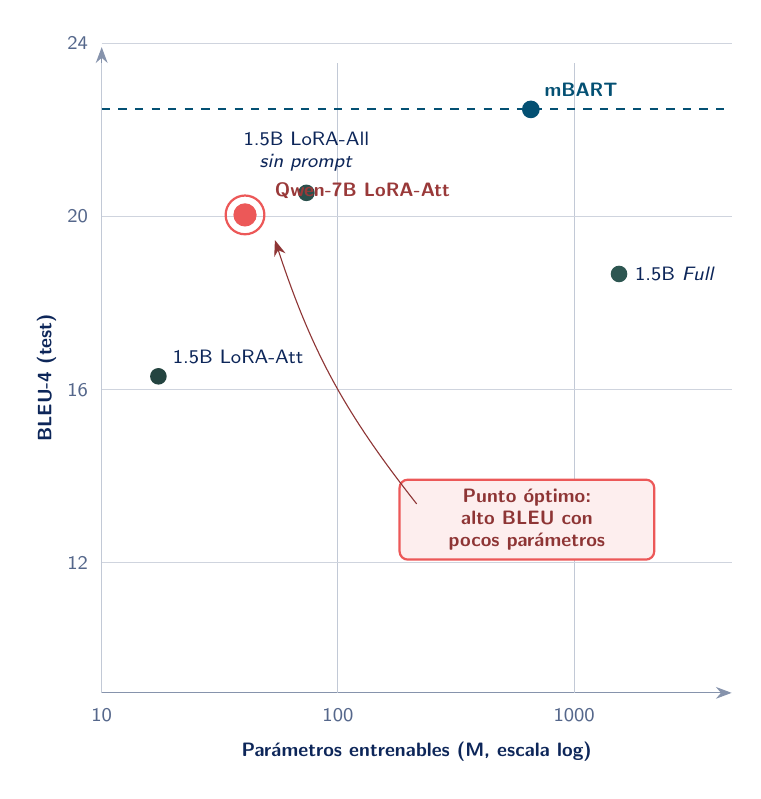
\begin{tikzpicture}[font=\sffamily]

% ejes
\draw[DarkBlue!50, -{Stealth[length=2mm]}] (0,0) -- (8.0,0);
\draw[DarkBlue!50, -{Stealth[length=2mm]}] (0,0) -- (0,8.2);
\node[font=\sffamily\scriptsize\bfseries, text=DarkBlue] at (4.0,-0.75)
    {Parámetros entrenables (M, escala log)};
\node[font=\sffamily\scriptsize\bfseries, text=DarkBlue, rotate=90] at (-0.7,4.0) {BLEU-4 (test)};

% ticks x en 10, 100, 1000 M -> log10 = 1,2,3 -> x=0,3,6
\foreach \p/\x in {10/0,100/3,1000/6}{
    \draw[DarkBlue!25] (\x,0)--(\x,8.0);
    \node[font=\sffamily\scriptsize, text=DarkBlue!70, anchor=north] at (\x,-0.08) {\p};
}
% ticks y
\foreach \b in {12,16,20,24}{
    \draw[DarkBlue!20] (0,{(\b-9)*0.55})--(8.0,{(\b-9)*0.55});
    \node[font=\sffamily\scriptsize, text=DarkBlue!70, anchor=east] at (-0.05,{(\b-9)*0.55}) {\b};
}

% linea mBART referencia
\draw[MediumBlue, dashed, thick] (0,{(22.48-9)*0.55}) -- (8.0,{(22.48-9)*0.55});

% puntos: x/y/color/etiqueta/anchor
% mBART: params 657.7 -> log 2.818 -> x=5.45 ; BLEU 22.48 -> y=7.41
\fill[MediumBlue] (5.45,7.41) circle (3.2pt);
\node[font=\sffamily\scriptsize\bfseries, text=MediumBlue, anchor=south west] at (5.5,7.45) {mBART};
% 1.5B Full: 1543.7 -> log 3.189 -> x=6.57 ; 18.68 -> y=5.32
\fill[MediumGreen!48!black] (6.57,5.32) circle (3.0pt);
\node[font=\sffamily\scriptsize, text=DarkBlue, anchor=west] at (6.65,5.32) {1.5B \emph{Full}};
% 1.5B LoRA-Att: 17.43 -> log 1.241 -> x=0.72 ; 16.31 -> y=4.02
\fill[MediumGreen!38!black] (0.72,4.02) circle (3.0pt);
\node[font=\sffamily\scriptsize, text=DarkBlue, anchor=south west] at (0.78,4.06) {1.5B LoRA-Att};
% 1.5B LoRA-All (sin prompt): 73.86 -> log 1.868 -> x=2.60 ; 20.55 -> y=6.35
\fill[MediumGreen!45!black] (2.60,6.35) circle (3.0pt);
\node[font=\sffamily\scriptsize, text=DarkBlue, anchor=south, align=center] at (2.60,6.5)
    {1.5B LoRA-All\\\emph{sin prompt}};
% 7B LoRA-Att: 40.37 -> log 1.606 -> x=1.82 ; 20.03 -> y=6.07  (SWEET SPOT)
\fill[MediumRed] (1.82,6.07) circle (4.2pt);
\draw[MediumRed, thick] (1.82,6.07) circle (7pt);
\node[font=\sffamily\scriptsize\bfseries, text=MediumRed!65!black, anchor=south west] at (2.0,6.15)
    {\;Qwen-7B LoRA-Att};

% callout sweet spot
\node[draw=MediumRed, thick, rounded corners=3pt, fill=MediumRed!10, text=MediumRed!60!black,
      font=\sffamily\scriptsize\bfseries, align=center, text width=3.0cm] at (5.4,2.2)
    {Punto óptimo:\\ alto BLEU con pocos parámetros};
\draw[-{Stealth[length=2mm]}, MediumRed!60!black] (4.0,2.4) to[bend left=10] (2.2,5.75);

\end{tikzpicture}
\end{document}
